\documentclass[twoside]{book}

% Packages required by doxygen
\usepackage{fixltx2e}
\usepackage{calc}
\usepackage{doxygen}
\usepackage[export]{adjustbox} % also loads graphicx
\usepackage{graphicx}
\usepackage[utf8]{inputenc}
\usepackage{makeidx}
\usepackage{multicol}
\usepackage{multirow}
\PassOptionsToPackage{warn}{textcomp}
\usepackage{textcomp}
\usepackage[nointegrals]{wasysym}
\usepackage[table]{xcolor}

% Font selection
\usepackage[T1]{fontenc}
\usepackage[scaled=.90]{helvet}
\usepackage{courier}
\usepackage{amssymb}
\usepackage{sectsty}
\renewcommand{\familydefault}{\sfdefault}
\allsectionsfont{%
  \fontseries{bc}\selectfont%
  \color{darkgray}%
}
\renewcommand{\DoxyLabelFont}{%
  \fontseries{bc}\selectfont%
  \color{darkgray}%
}
\newcommand{\+}{\discretionary{\mbox{\scriptsize$\hookleftarrow$}}{}{}}

% Page & text layout
\usepackage{geometry}
\geometry{%
  a4paper,%
  top=2.5cm,%
  bottom=2.5cm,%
  left=2.5cm,%
  right=2.5cm%
}
\tolerance=750
\hfuzz=15pt
\hbadness=750
\setlength{\emergencystretch}{15pt}
\setlength{\parindent}{0cm}
\setlength{\parskip}{3ex plus 2ex minus 2ex}
\makeatletter
\renewcommand{\paragraph}{%
  \@startsection{paragraph}{4}{0ex}{-1.0ex}{1.0ex}{%
    \normalfont\normalsize\bfseries\SS@parafont%
  }%
}
\renewcommand{\subparagraph}{%
  \@startsection{subparagraph}{5}{0ex}{-1.0ex}{1.0ex}{%
    \normalfont\normalsize\bfseries\SS@subparafont%
  }%
}
\makeatother

% Headers & footers
\usepackage{fancyhdr}
\pagestyle{fancyplain}
\fancyhead[LE]{\fancyplain{}{\bfseries\thepage}}
\fancyhead[CE]{\fancyplain{}{}}
\fancyhead[RE]{\fancyplain{}{\bfseries\leftmark}}
\fancyhead[LO]{\fancyplain{}{\bfseries\rightmark}}
\fancyhead[CO]{\fancyplain{}{}}
\fancyhead[RO]{\fancyplain{}{\bfseries\thepage}}
\fancyfoot[LE]{\fancyplain{}{}}
\fancyfoot[CE]{\fancyplain{}{}}
\fancyfoot[RE]{\fancyplain{}{\bfseries\scriptsize Generated by Doxygen }}
\fancyfoot[LO]{\fancyplain{}{\bfseries\scriptsize Generated by Doxygen }}
\fancyfoot[CO]{\fancyplain{}{}}
\fancyfoot[RO]{\fancyplain{}{}}
\renewcommand{\footrulewidth}{0.4pt}
\renewcommand{\chaptermark}[1]{%
  \markboth{#1}{}%
}
\renewcommand{\sectionmark}[1]{%
  \markright{\thesection\ #1}%
}

% Indices & bibliography
\usepackage{natbib}
\usepackage[titles]{tocloft}
\setcounter{tocdepth}{3}
\setcounter{secnumdepth}{5}
\makeindex

% Hyperlinks (required, but should be loaded last)
\usepackage{ifpdf}
\ifpdf
  \usepackage[pdftex,pagebackref=true]{hyperref}
\else
  \usepackage[ps2pdf,pagebackref=true]{hyperref}
\fi
\hypersetup{%
  colorlinks=true,%
  linkcolor=blue,%
  citecolor=blue,%
  unicode%
}

% Custom commands
\newcommand{\clearemptydoublepage}{%
  \newpage{\pagestyle{empty}\cleardoublepage}%
}

\usepackage{caption}
\captionsetup{labelsep=space,justification=centering,font={bf},singlelinecheck=off,skip=4pt,position=top}

%===== C O N T E N T S =====

\begin{document}

% Titlepage & ToC
\hypersetup{pageanchor=false,
             bookmarksnumbered=true,
             pdfencoding=unicode
            }
\pagenumbering{alph}
\begin{titlepage}
\vspace*{7cm}
\begin{center}%
{\Large Trilinos Concept Map }\\
\vspace*{1cm}
{\large Generated by Doxygen 1.8.13}\\
\end{center}
\end{titlepage}
\clearemptydoublepage
\pagenumbering{roman}
\tableofcontents
\clearemptydoublepage
\pagenumbering{arabic}
\hypersetup{pageanchor=true}

%--- Begin generated contents ---
\chapter{Categories}
\label{md_markdown_categories}
\Hypertarget{md_markdown_categories}

\begin{DoxyImageNoCaption}
  \mbox{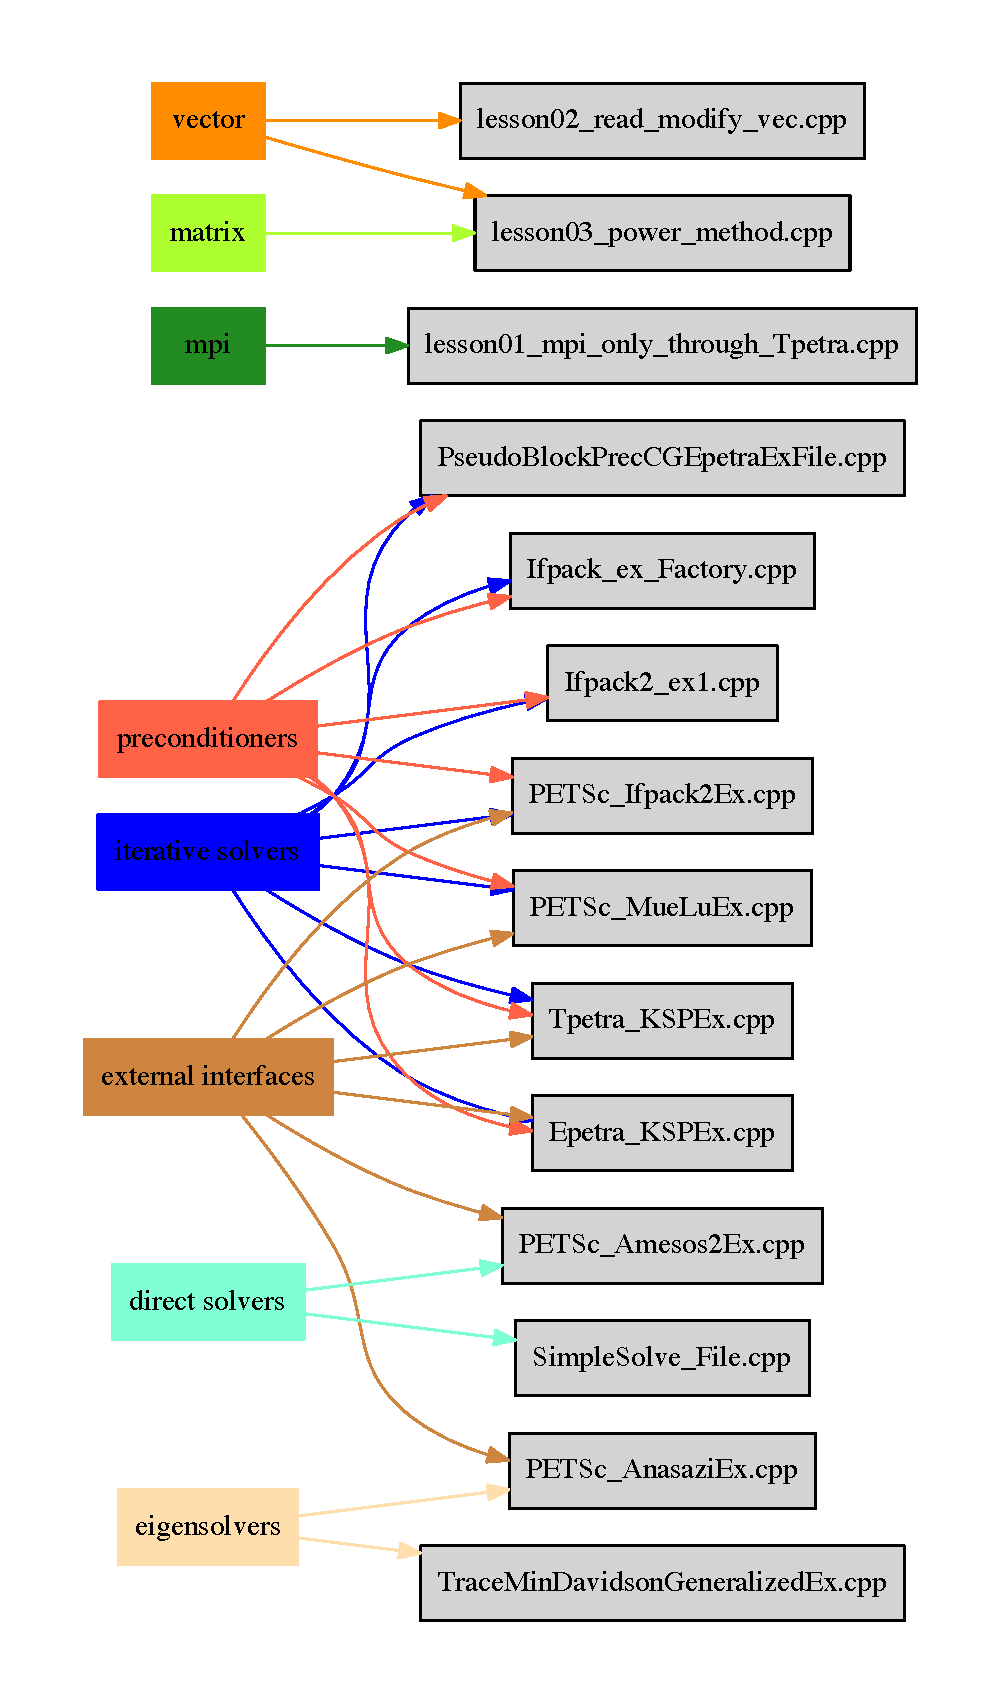
\includegraphics[width=\textwidth,height=\textheight/2,keepaspectratio=true]{dot_categories}}
\end{DoxyImageNoCaption}
 
\chapter{Category\+: Direct solvers}
\label{md_markdown_category_direct_solvers}
\Hypertarget{md_markdown_category_direct_solvers}

\begin{DoxyImageNoCaption}
  \mbox{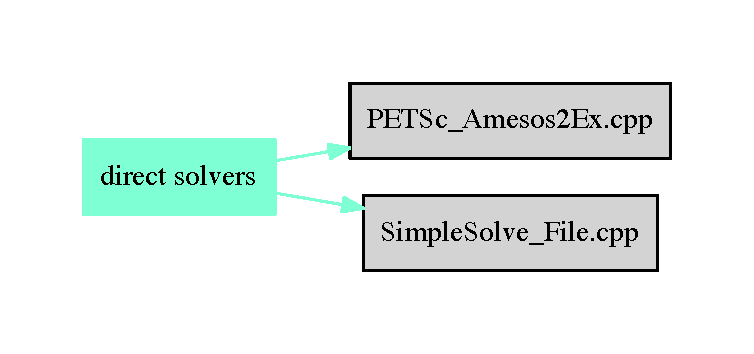
\includegraphics[width=\textwidth,height=\textheight/2,keepaspectratio=true]{dot_category_direct_solvers}}
\end{DoxyImageNoCaption}
 
\chapter{Category\+: Eigensolvers}
\label{md_markdown_category_eigensolvers}
\Hypertarget{md_markdown_category_eigensolvers}

\begin{DoxyImageNoCaption}
  \mbox{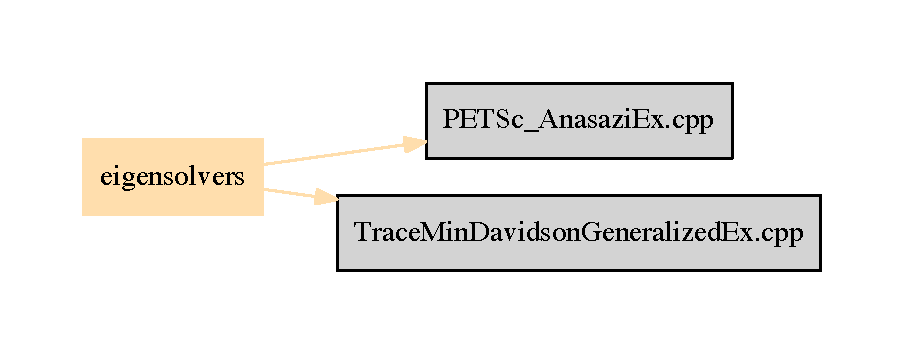
\includegraphics[width=\textwidth,height=\textheight/2,keepaspectratio=true]{dot_category_eigensolvers}}
\end{DoxyImageNoCaption}
 
\chapter{Category\+: External interfaces}
\label{md_markdown_category_external_interfaces}
\Hypertarget{md_markdown_category_external_interfaces}

\begin{DoxyImageNoCaption}
  \mbox{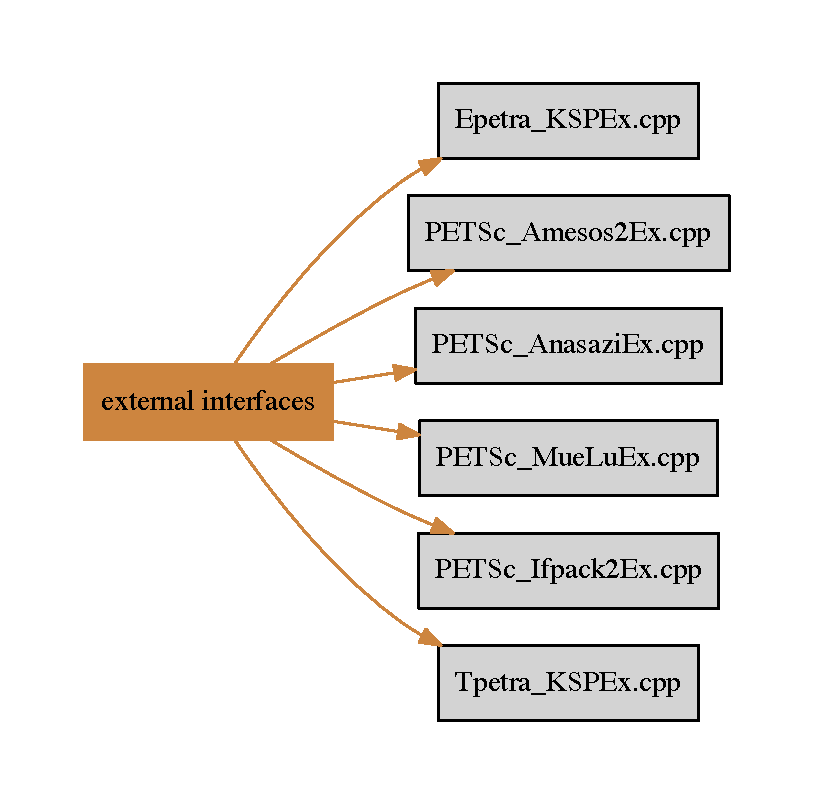
\includegraphics[width=\textwidth,height=\textheight/2,keepaspectratio=true]{dot_category_external_interfaces}}
\end{DoxyImageNoCaption}
 
\chapter{Category\+: Iterative solvers}
\label{md_markdown_category_iterative_solvers}
\Hypertarget{md_markdown_category_iterative_solvers}

\begin{DoxyImageNoCaption}
  \mbox{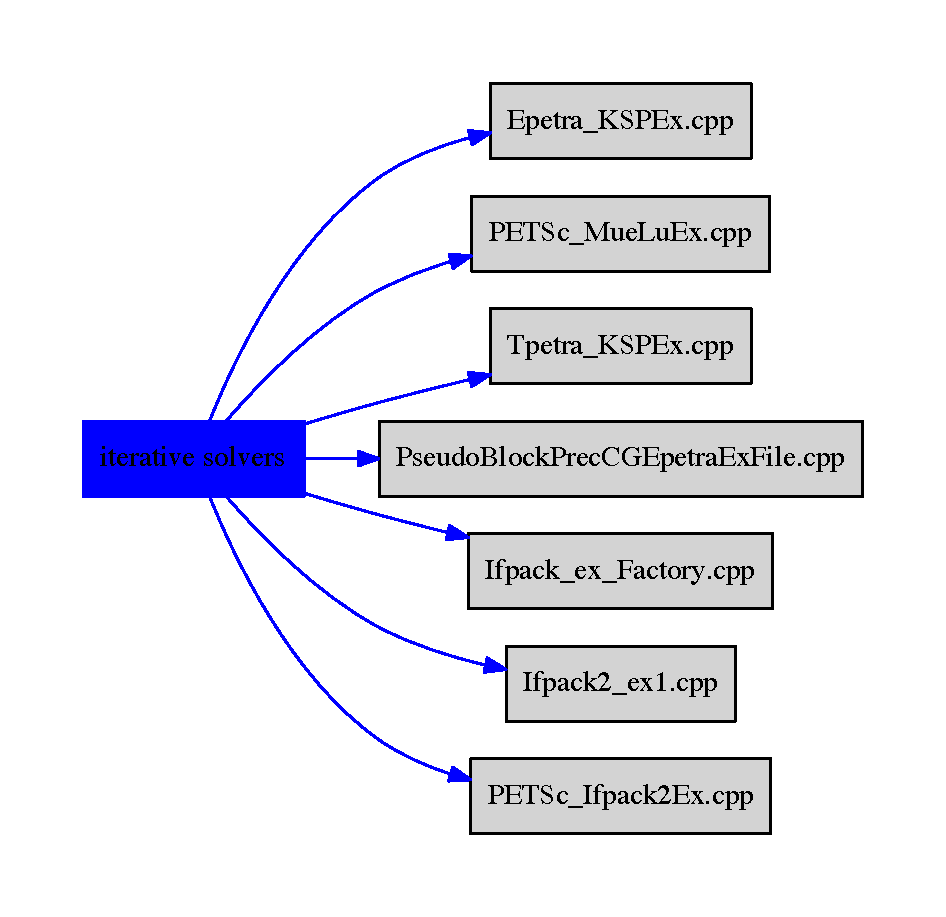
\includegraphics[width=\textwidth,height=\textheight/2,keepaspectratio=true]{dot_category_iterative_solvers}}
\end{DoxyImageNoCaption}
 
\chapter{Category\+: Matrix}
\label{md_markdown_category_matrix}
\Hypertarget{md_markdown_category_matrix}

\begin{DoxyImageNoCaption}
  \mbox{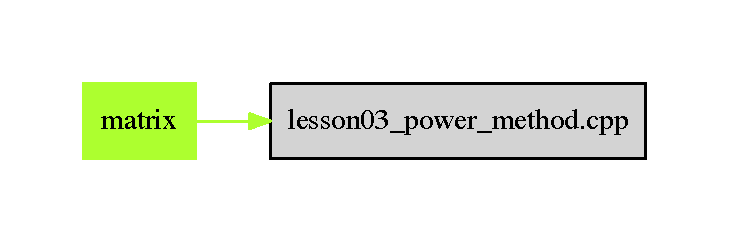
\includegraphics[width=\textwidth,height=\textheight/2,keepaspectratio=true]{dot_category_matrix}}
\end{DoxyImageNoCaption}
 
\chapter{Category\+: M\+PI}
\label{md_markdown_category_mpi}
\Hypertarget{md_markdown_category_mpi}

\begin{DoxyImageNoCaption}
  \mbox{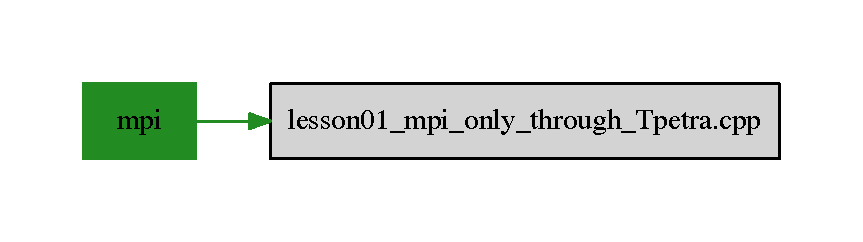
\includegraphics[width=\textwidth,height=\textheight/2,keepaspectratio=true]{dot_category_mpi}}
\end{DoxyImageNoCaption}
 
\chapter{Category\+: Preconditioners}
\label{md_markdown_category_preconditioners}
\Hypertarget{md_markdown_category_preconditioners}

\begin{DoxyImageNoCaption}
  \mbox{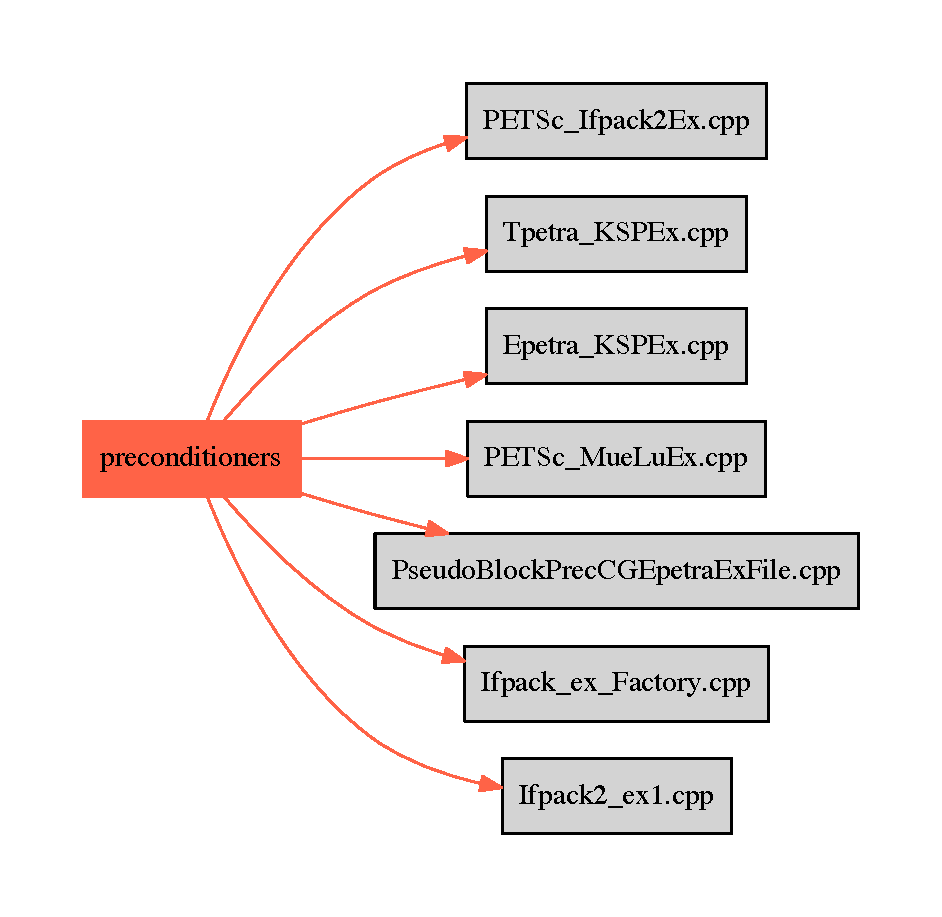
\includegraphics[width=\textwidth,height=\textheight/2,keepaspectratio=true]{dot_category_preconditioners}}
\end{DoxyImageNoCaption}
 
\chapter{Category\+: Vector}
\label{md_markdown_category_vector}
\Hypertarget{md_markdown_category_vector}

\begin{DoxyImageNoCaption}
  \mbox{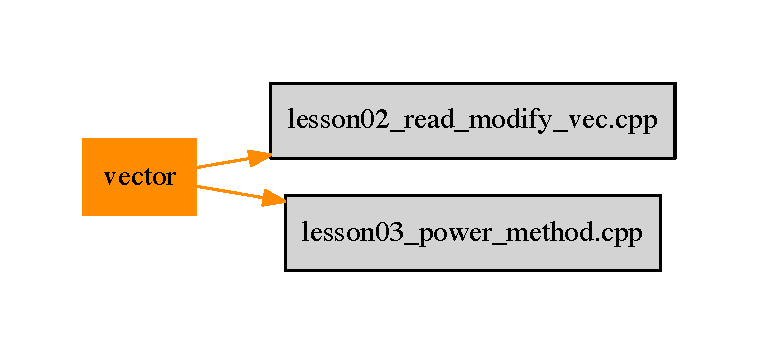
\includegraphics[width=\textwidth,height=\textheight/2,keepaspectratio=true]{dot_category_vector}}
\end{DoxyImageNoCaption}
 
\chapter{Trilinos Map}
\label{md_markdown_map}
\Hypertarget{md_markdown_map}

\begin{DoxyImageNoCaption}
  \mbox{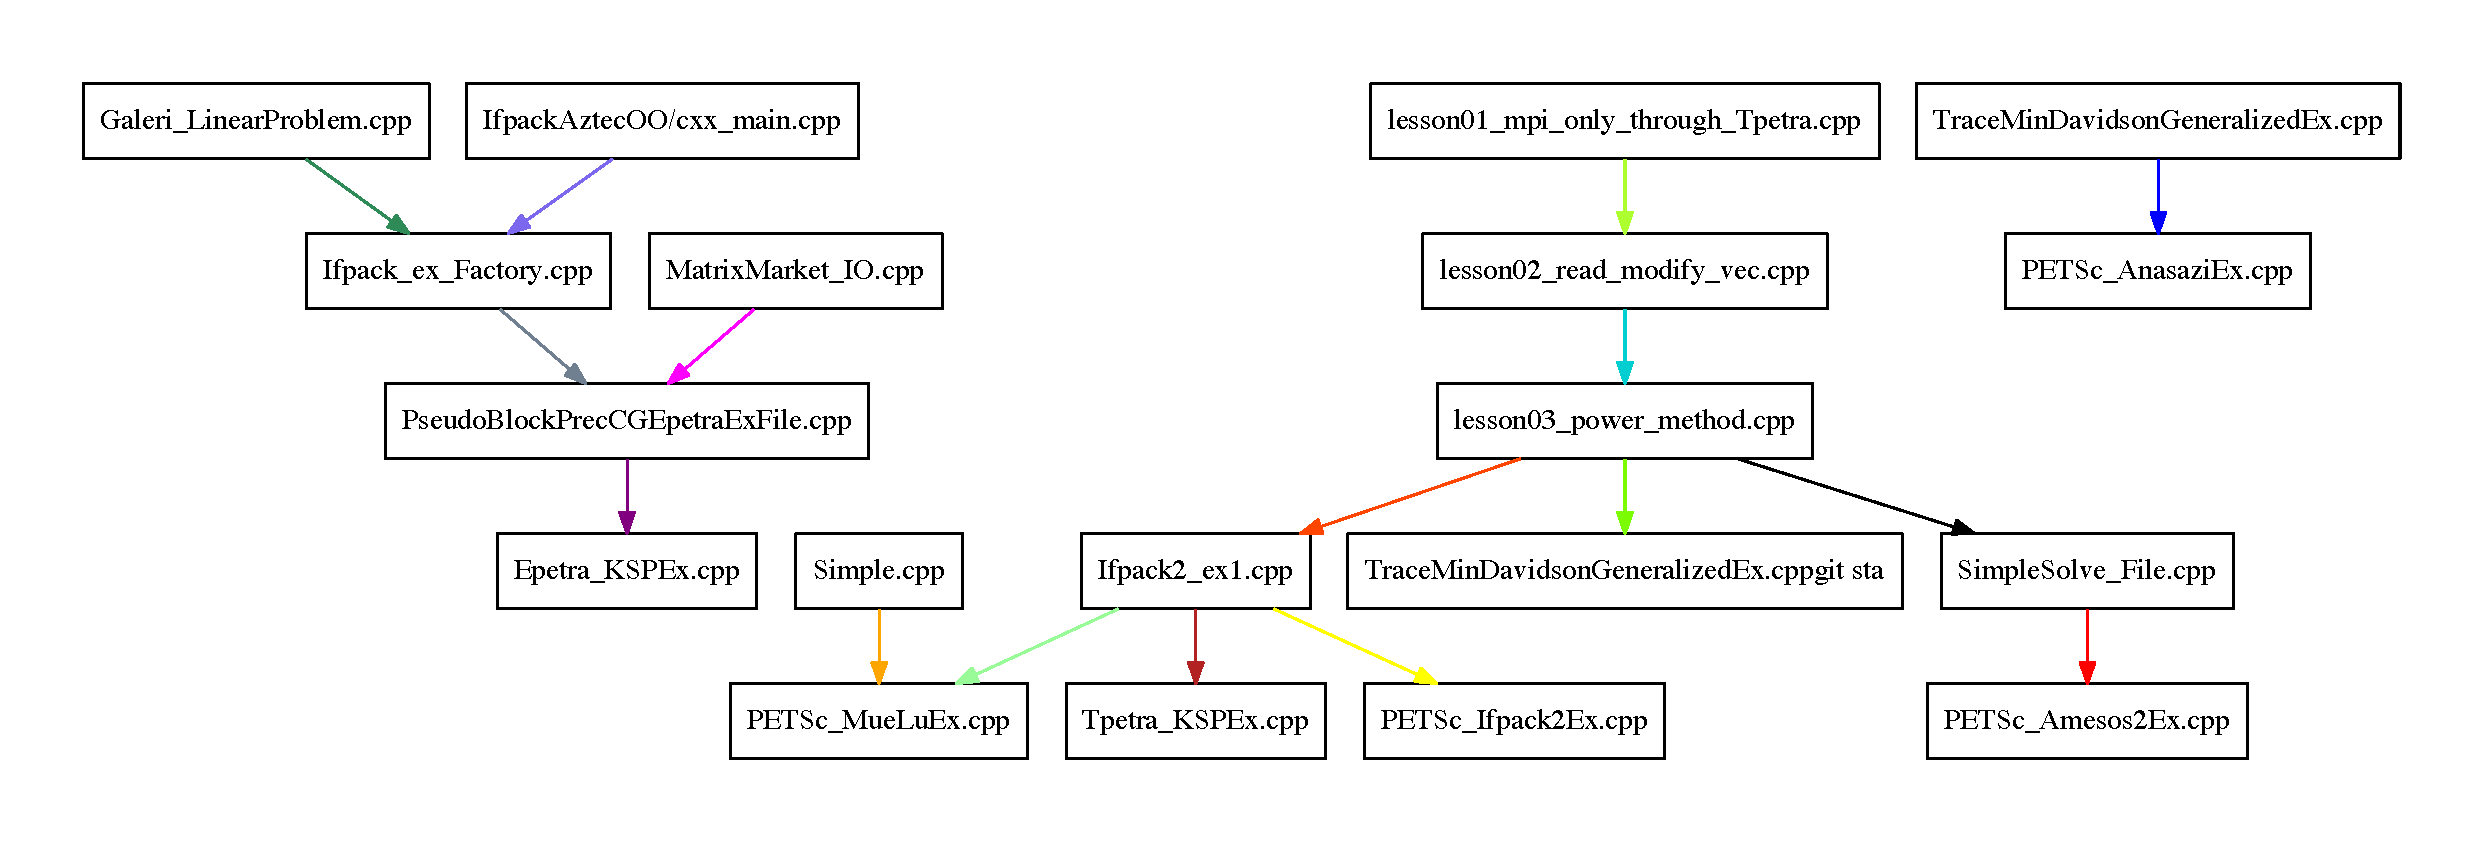
\includegraphics[width=\textwidth,height=\textheight/2,keepaspectratio=true]{dot_map}}
\end{DoxyImageNoCaption}
 
\chapter{Topic\+: Creating linear algebra objects}
\label{md_markdown_topic_creating_linear_algebra_objects}
\Hypertarget{md_markdown_topic_creating_linear_algebra_objects}

\begin{DoxyImageNoCaption}
  \mbox{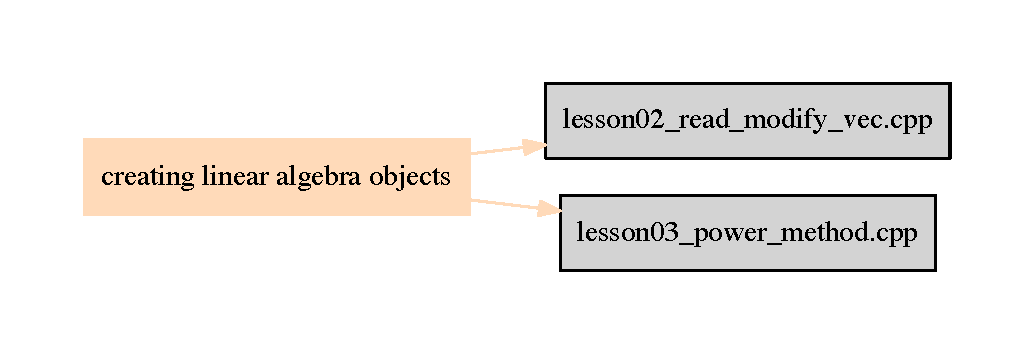
\includegraphics[width=\textwidth,height=\textheight/2,keepaspectratio=true]{dot_topic_creating_linear_algebra_objects}}
\end{DoxyImageNoCaption}
 
\chapter{Topic\+: Setting up parallel code}
\label{md_markdown_topic_setting_up_parallel_code}
\Hypertarget{md_markdown_topic_setting_up_parallel_code}

\begin{DoxyImageNoCaption}
  \mbox{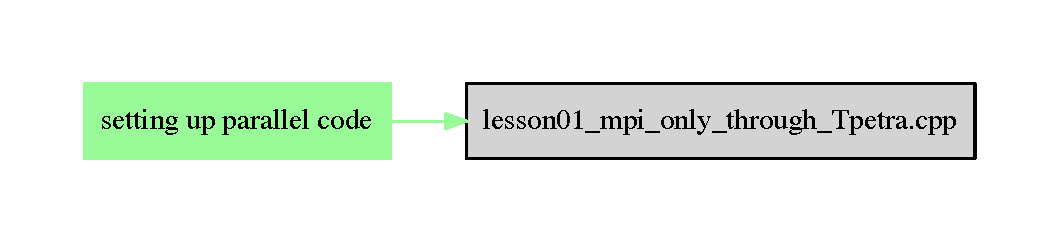
\includegraphics[width=\textwidth,height=\textheight/2,keepaspectratio=true]{dot_topic_setting_up_parallel_code}}
\end{DoxyImageNoCaption}
 
\chapter{Topic\+: Solve a linear system}
\label{md_markdown_topic_solve_a_linear_system}
\Hypertarget{md_markdown_topic_solve_a_linear_system}

\begin{DoxyImageNoCaption}
  \mbox{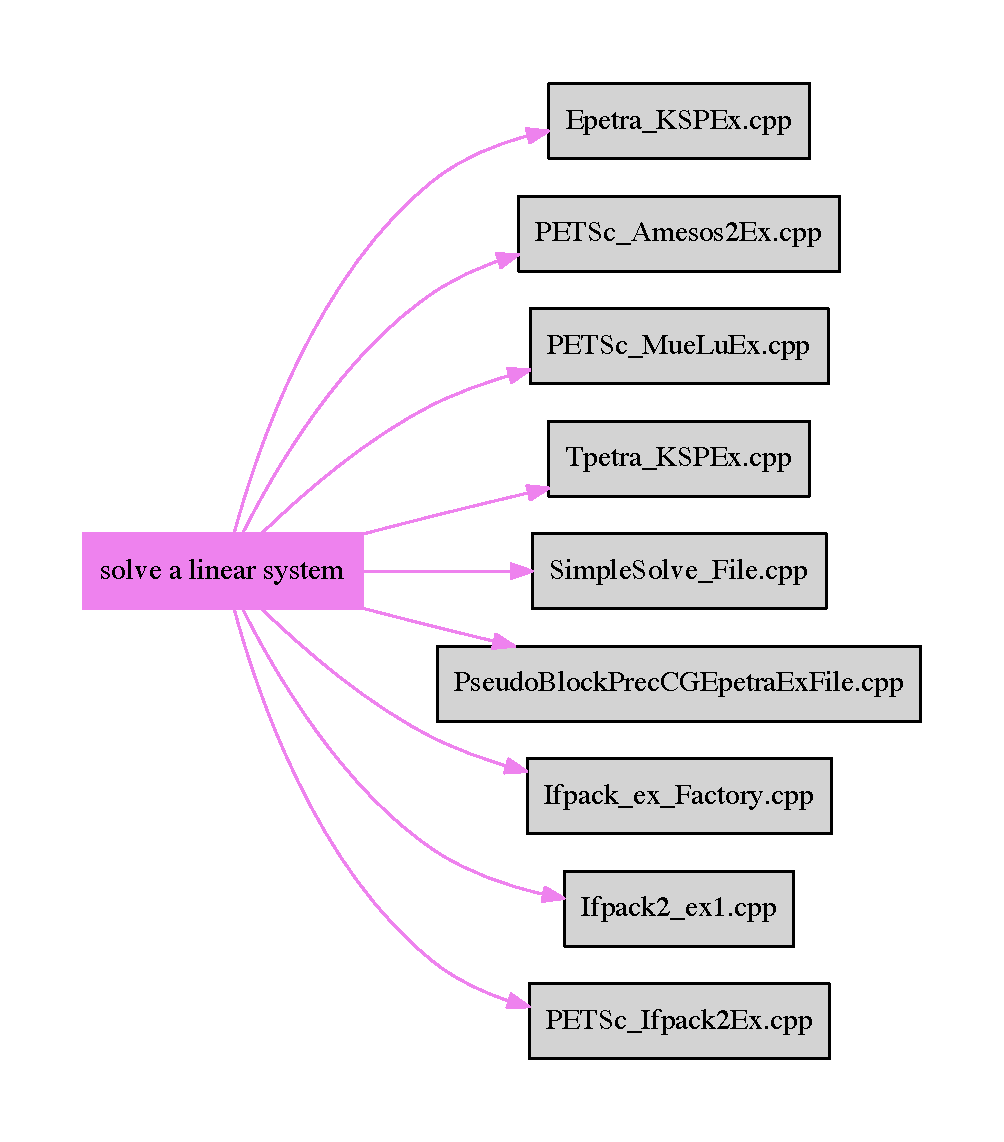
\includegraphics[width=\textwidth,height=\textheight/2,keepaspectratio=true]{dot_topic_solve_a_linear_system}}
\end{DoxyImageNoCaption}
 
\chapter{Topic\+: Solve an eigenvalue problem}
\label{md_markdown_topic_solve_an_eigenvalue_problem}
\Hypertarget{md_markdown_topic_solve_an_eigenvalue_problem}

\begin{DoxyImageNoCaption}
  \mbox{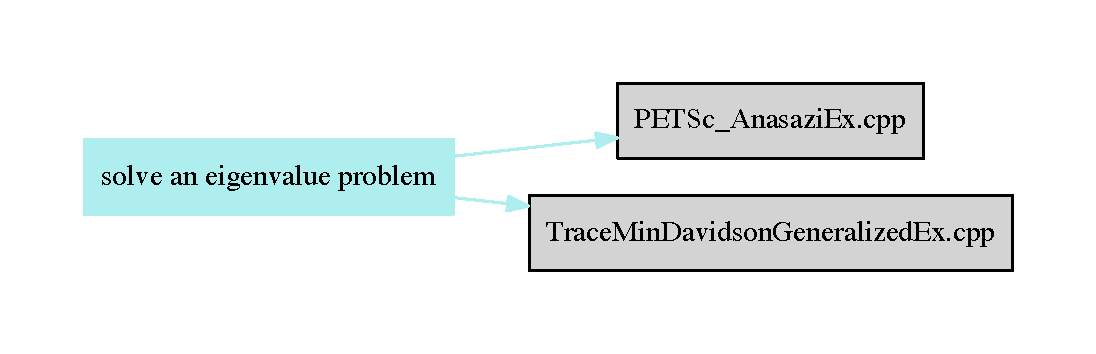
\includegraphics[width=\textwidth,height=\textheight/2,keepaspectratio=true]{dot_topic_solve_an_eigenvalue_problem}}
\end{DoxyImageNoCaption}
 
\chapter{Topics}
\label{md_markdown_topics}
\Hypertarget{md_markdown_topics}

\begin{DoxyImageNoCaption}
  \mbox{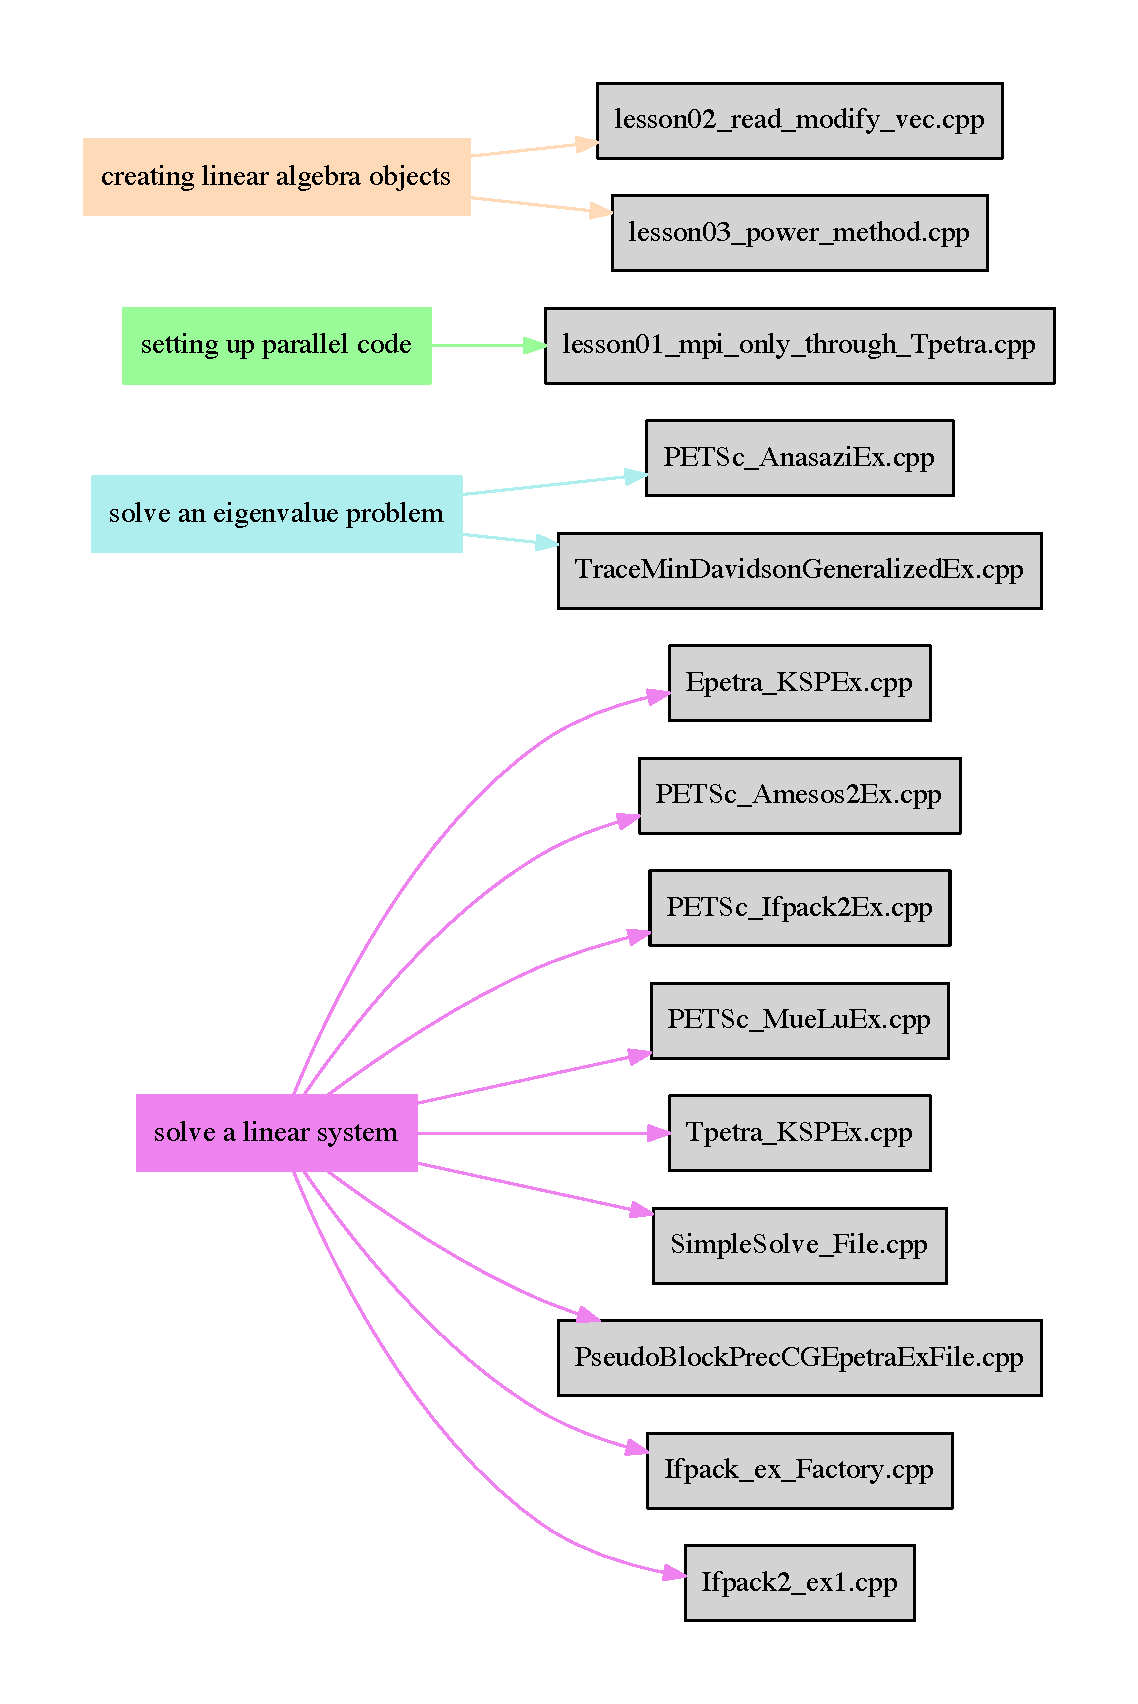
\includegraphics[width=\textwidth,height=\textheight/2,keepaspectratio=true]{dot_topics}}
\end{DoxyImageNoCaption}
 
\chapter{Namespace Index}
\section{Namespace List}
Here is a list of all namespaces with brief descriptions\+:\begin{DoxyCompactList}
\item\contentsline{section}{\hyperlink{namespacesubfiles__generator}{subfiles\+\_\+generator} }{\pageref{namespacesubfiles__generator}}{}
\end{DoxyCompactList}

\chapter{File Index}
\section{File List}
Here is a list of all files with brief descriptions\+:\begin{DoxyCompactList}
\item\contentsline{section}{markdown/\hyperlink{subfiles__generator_8py}{subfiles\+\_\+generator.\+py} }{\pageref{subfiles__generator_8py}}{}
\end{DoxyCompactList}

\chapter{Namespace Documentation}
\hypertarget{namespacesubfiles__generator}{}\section{subfiles\+\_\+generator Namespace Reference}
\label{namespacesubfiles__generator}\index{subfiles\+\_\+generator@{subfiles\+\_\+generator}}
\subsection*{Functions}
\begin{DoxyCompactItemize}
\item 
def \hyperlink{namespacesubfiles__generator_ae4057a32539f835494f8bfcc388bf072}{read\+\_\+file} ()
\end{DoxyCompactItemize}


\subsection{Function Documentation}
\mbox{\Hypertarget{namespacesubfiles__generator_ae4057a32539f835494f8bfcc388bf072}\label{namespacesubfiles__generator_ae4057a32539f835494f8bfcc388bf072}} 
\index{subfiles\+\_\+generator@{subfiles\+\_\+generator}!read\+\_\+file@{read\+\_\+file}}
\index{read\+\_\+file@{read\+\_\+file}!subfiles\+\_\+generator@{subfiles\+\_\+generator}}
\subsubsection{\texorpdfstring{read\+\_\+file()}{read\_file()}}
{\footnotesize\ttfamily def subfiles\+\_\+generator.\+read\+\_\+file (\begin{DoxyParamCaption}{ }\end{DoxyParamCaption})}


\chapter{File Documentation}
\hypertarget{categories_8md}{}\section{markdown/categories.md File Reference}
\label{categories_8md}\index{markdown/categories.\+md@{markdown/categories.\+md}}

\hypertarget{category__direct__solvers_8md}{}\section{markdown/category\+\_\+direct\+\_\+solvers.md File Reference}
\label{category__direct__solvers_8md}\index{markdown/category\+\_\+direct\+\_\+solvers.\+md@{markdown/category\+\_\+direct\+\_\+solvers.\+md}}

\hypertarget{category__eigensolvers_8md}{}\section{markdown/category\+\_\+eigensolvers.md File Reference}
\label{category__eigensolvers_8md}\index{markdown/category\+\_\+eigensolvers.\+md@{markdown/category\+\_\+eigensolvers.\+md}}

\hypertarget{category__external__interfaces_8md}{}\section{markdown/category\+\_\+external\+\_\+interfaces.md File Reference}
\label{category__external__interfaces_8md}\index{markdown/category\+\_\+external\+\_\+interfaces.\+md@{markdown/category\+\_\+external\+\_\+interfaces.\+md}}

\hypertarget{category__iterative__solvers_8md}{}\section{markdown/category\+\_\+iterative\+\_\+solvers.md File Reference}
\label{category__iterative__solvers_8md}\index{markdown/category\+\_\+iterative\+\_\+solvers.\+md@{markdown/category\+\_\+iterative\+\_\+solvers.\+md}}

\hypertarget{category__matrix_8md}{}\section{markdown/category\+\_\+matrix.md File Reference}
\label{category__matrix_8md}\index{markdown/category\+\_\+matrix.\+md@{markdown/category\+\_\+matrix.\+md}}

\hypertarget{category__mpi_8md}{}\section{markdown/category\+\_\+mpi.md File Reference}
\label{category__mpi_8md}\index{markdown/category\+\_\+mpi.\+md@{markdown/category\+\_\+mpi.\+md}}

\hypertarget{category__preconditioners_8md}{}\section{markdown/category\+\_\+preconditioners.md File Reference}
\label{category__preconditioners_8md}\index{markdown/category\+\_\+preconditioners.\+md@{markdown/category\+\_\+preconditioners.\+md}}

\hypertarget{category__vector_8md}{}\section{markdown/category\+\_\+vector.md File Reference}
\label{category__vector_8md}\index{markdown/category\+\_\+vector.\+md@{markdown/category\+\_\+vector.\+md}}

\hypertarget{map_8md}{}\section{markdown/map.md File Reference}
\label{map_8md}\index{markdown/map.\+md@{markdown/map.\+md}}

\hypertarget{subfiles__generator_8py}{}\section{markdown/subfiles\+\_\+generator.py File Reference}
\label{subfiles__generator_8py}\index{markdown/subfiles\+\_\+generator.\+py@{markdown/subfiles\+\_\+generator.\+py}}
\subsection*{Namespaces}
\begin{DoxyCompactItemize}
\item 
 \hyperlink{namespacesubfiles__generator}{subfiles\+\_\+generator}
\end{DoxyCompactItemize}
\subsection*{Functions}
\begin{DoxyCompactItemize}
\item 
def \hyperlink{namespacesubfiles__generator_ae4057a32539f835494f8bfcc388bf072}{subfiles\+\_\+generator.\+read\+\_\+file} ()
\end{DoxyCompactItemize}

\hypertarget{topic__creating__linear__algebra__objects_8md}{}\section{markdown/topic\+\_\+creating\+\_\+linear\+\_\+algebra\+\_\+objects.md File Reference}
\label{topic__creating__linear__algebra__objects_8md}\index{markdown/topic\+\_\+creating\+\_\+linear\+\_\+algebra\+\_\+objects.\+md@{markdown/topic\+\_\+creating\+\_\+linear\+\_\+algebra\+\_\+objects.\+md}}

\hypertarget{topic__setting__up__parallel__code_8md}{}\section{markdown/topic\+\_\+setting\+\_\+up\+\_\+parallel\+\_\+code.md File Reference}
\label{topic__setting__up__parallel__code_8md}\index{markdown/topic\+\_\+setting\+\_\+up\+\_\+parallel\+\_\+code.\+md@{markdown/topic\+\_\+setting\+\_\+up\+\_\+parallel\+\_\+code.\+md}}

\hypertarget{topic__solve__a__linear__system_8md}{}\section{markdown/topic\+\_\+solve\+\_\+a\+\_\+linear\+\_\+system.md File Reference}
\label{topic__solve__a__linear__system_8md}\index{markdown/topic\+\_\+solve\+\_\+a\+\_\+linear\+\_\+system.\+md@{markdown/topic\+\_\+solve\+\_\+a\+\_\+linear\+\_\+system.\+md}}

\hypertarget{topic__solve__an__eigenvalue__problem_8md}{}\section{markdown/topic\+\_\+solve\+\_\+an\+\_\+eigenvalue\+\_\+problem.md File Reference}
\label{topic__solve__an__eigenvalue__problem_8md}\index{markdown/topic\+\_\+solve\+\_\+an\+\_\+eigenvalue\+\_\+problem.\+md@{markdown/topic\+\_\+solve\+\_\+an\+\_\+eigenvalue\+\_\+problem.\+md}}

\hypertarget{topics_8md}{}\section{markdown/topics.md File Reference}
\label{topics_8md}\index{markdown/topics.\+md@{markdown/topics.\+md}}

%--- End generated contents ---

% Index
\backmatter
\newpage
\phantomsection
\clearemptydoublepage
\addcontentsline{toc}{chapter}{Index}
\printindex

\end{document}
